\documentclass{article}
\usepackage[utf8]{inputenc}
\usepackage{setspace}
\usepackage{graphicx}
\usepackage{dirtree}
\usepackage[hang]{footmisc}
\usepackage{vhistory}
\renewcommand{\hangfootparskip}{10pt}
\setlength{\skip\footins}{1cm}
\setlength{\parskip}{1em}
\usepackage[a4paper, total={6in, 8in}]{geometry}


\title{%
Upgrading Lustre File System with Minimal Downtime\\
\large Zenuity Oden Cluster (NGSC)}
\author{Carlos Thomaz - cthomaz@ddn.com}
\date{\today}
\begin{document}

\maketitle


\begin{center}
    
\includegraphics[scale=0.14]{logo.png}\\[1cm] 
\end{center}

\newpage

\begin{versionhistory}
    \vhEntry{Draft}{05.12.20}{CT}{DRAFT - Initial version}
\end{versionhistory}


\newpage
\section{Introduction}
This document describes possible Lustre upgrades Upgrades procedures aiming reduction down-time and problem  mitigation strategy during upgrades. 

\section{Upgrades - Definition}
Upgrades are usually referred to either the increasing of resources in an existing file system or to the process of update resources (hardware or software firmware). Both actions may happen in the same time, taking advantage of system's maintenance window. For this document we will refer as \textbf{Upgrades} the action taken to add more hardware and software resources, increasing the performance and capacity of the file systems. We will refer to \textbf{Updates} the action of leveling software and hardware firmware to newer versions and/or implementing patches and bug fixes to the solution.

There's also chances the system(s) will be put under maintenance for the purpose of Hardware replacement. We usually refer to this action as \textbf{Hardware maintenance window}.

\subsection{System upgrades - adding additional resources}
Systems upgrades will be triggered when a file system capacity is close to full, performance of the current file system is not enough or due a potential cyclic planed upgrade.\footnote{For instance, some projects forecast hardware upgrades in advanced, regardless if the capacity or performance requires it. Usually the use of resources are imminent and such upgrades are taken pro-actively to avoid an unexpected resource shortage}

\subsubsection{Planed downtime}
Eight (8) hours a month will be given to general maintenance purposes. Hardware and Software upgrades may use this planed downtime to \textbf{complete} such tasks. The planed downtime will likely be used for multiple concurrent tasks, so a filesystem maintenance must be agreed in advance since possible tasks may require access to data. 

\subsubsection{Scheduling Upgrades}

Hardware upgrades usually require a detailed planing for multiple stages that includes but not limited to:
\begin{itemize}
    \item Order entry
    \item Shipping and receiving
    \item Hardware installation (commonly referred as Rack and Stacking)
    \item Offline Hardware installation
    \item Software installation and customization
    \item Resource Insertion
    \item Rollout
\end{itemize}

For simplification purposes it will be considered that Order entry and Shipping and Receiving are tasks to be sorted independently, so the planing will be designed from the Rack and Stacking initial date and beyond.

\begin{figure}
    \centering
    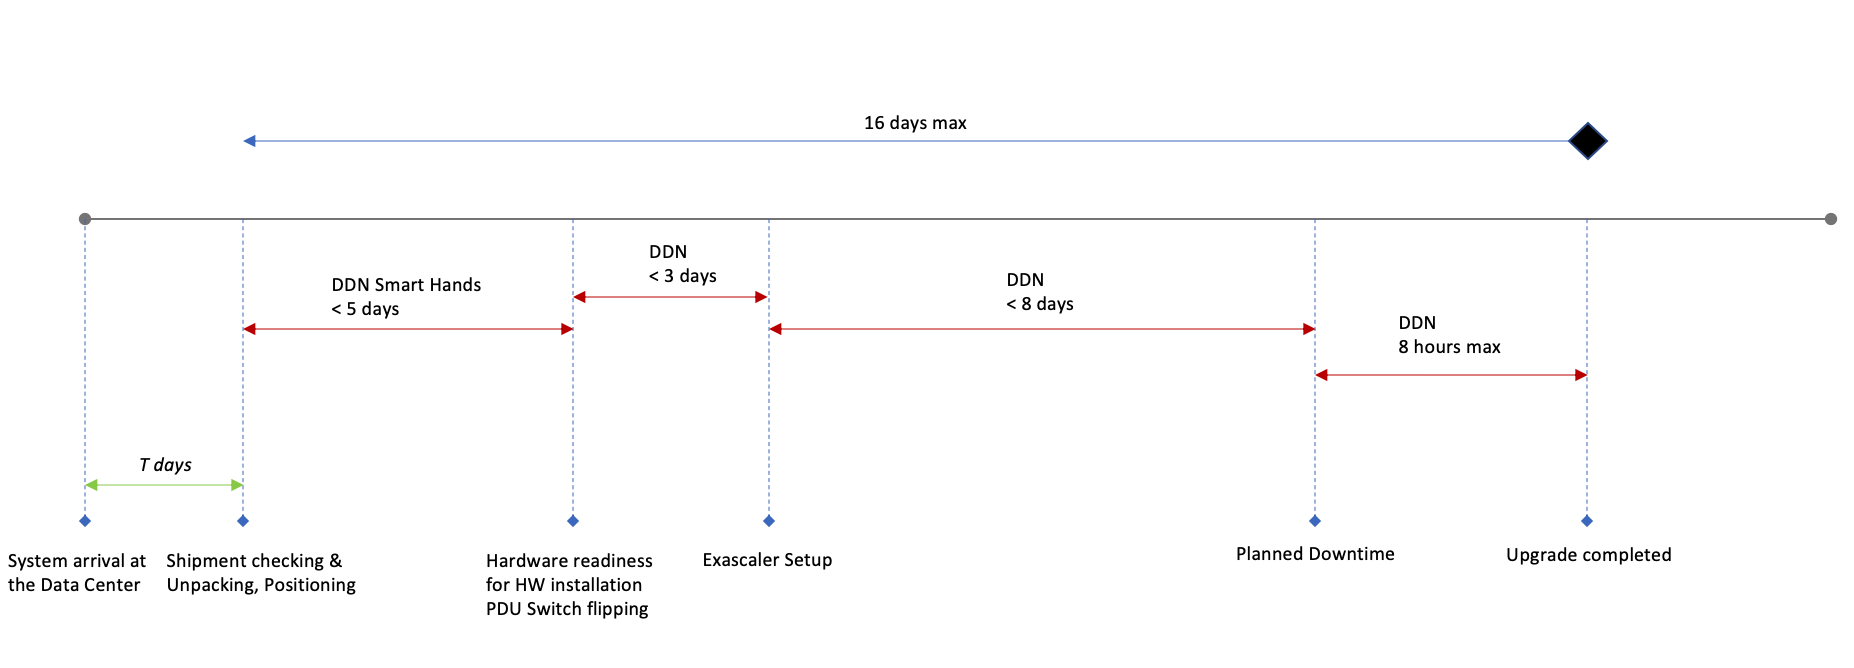
\includegraphics[scale=0.4]{ES-upgrade-timeline.png}
    \caption{Exascaler Upgrade Timeline}
    \label{fig:es-upgrade-timeline-v2}
\end{figure}

\subsubsection{Pre-requisites}
It is assumed a set of pre-requisites to be agreed and implemented before the upgrade process start. These pre-requisites are concurrent and do not interfere on the production system and will be done in parallel not affecting downtime. Similarly to the initial filesystem installation, a checklist will be produced for each stage of the upgrade (e.g.: what is needed to be ready before receiving an upgrade kit or before start installing the hardware or software). Those activities are laid out linearly intentionally. However, there are sub tasks on each stage that may be executed in parallel.

\subsubsection{Planning downtime}
The timeline\footnote{Times are subjected to adjustments upon refinement} on Figure \ref{fig:es-upgrade-timeline-v2} suggest that a minimum of 16 days to be accounted before commit to an upgrade. Since the planed downtime will a date defined in advance, it's recommended to calculate backwards to define the critical dates for each sub-phase be completed. 

\subsubsection{Remediation and Fallback plan}
The goal is to minimize the chances of failures during the planed downtime. However it will be necessary to create a fallback or bail-out plan. These criterias are not yet clear, but will be required to be set as milestones where subsequent tasks will rely on. One example is DOA and lack of spare part for on-site replacement. This hypothetical scenario may lead to a bail-out depending on how the new spare part is shipped. Another example is a logical error when preparing the new upgrade units for go-live. A software bug may be found requiring a bail-out as well. A more serious scenario is a failure within the 8 hours planed downtime, requiring a fall-back plan to re-establish the system to the state prior the beginning of the upgrade (undo). In such cases, the availability and file system reliability are prioritized.

\subsection{System updates - leveling software and firmware and applying patches and fixes}
AS mentioned previously most of the tasks will be done concurrently. That includes the software installation on the new DDN Exascaler \textit{stacks} and possible hardware firmware updates. Considering a planed downtime, in a moment when the clock start counting, the existing file system will be placed in maintenance mode, namespace will be unmounted and hardware firmware upgrades will be applied (if necessary). There are two possible scenarios for the system upgrades.
\subsubsection{Upgrades that require an Exascaler update}
In the moment of planing for upgrade, it may be desired or needed to also plan for a software upgrade, meaning, hardware will be added to aggregate capacity and performance, but also Exascaler may be required to be upgrade (e.g.: need of fixing a bug or a possible new feature). In this scenario, the software upgrade is required to be prioritized. The tasks done before the planed downtime will assume the new Exascaler version. Once the system is placed in maintenance mode, the existing building blocks will be updated and once is confirmed to be successfully executed, we will proceed with the new hardware addition.

\subsubsection{Upgrades that doesn't require an Exascaler update}
In a more simplistic scenario, there will be no need of Exascaler update. In this case, the same version as the currenty running system will be installed and when the planed downtime start counting, the system will be place in maintenance mode and the new building blocks will be immediately added into the file system. This scenario is simpler and less risky.

\subsection{Versions and updates}
A proper risk analysis should be done during the upgrade plan. It is necessary to evaluate if an upgrade is required and what are the needs and risks associated with that. If a filesystem is running without issues and there's no new feature required, it is not recommended to plan for software upgrades. However, an outstanding bug or issue may require a sole software upgrade (not associated with a hardware upgrade).

\section{In production maintenance}
After a sucessfull upgrade or software update, it may be required to run a set of tasks with the system in production and concurrently with user's jobs. These tasks may include partial data re-balancing or data-redistribution. 

It is imperative to have a former decision on what strategy will be taken in consideration after an upgrade. If data re-balancing (full or partial) is required a set of tasks will be required to run for hours or even days after the physical / hardware upgrade concludes. As detailed on the File System Re-balancing strategies documentation, each possible alternative may affect the system availability and peroformance differently and must be agreed in advance. 

\end{document}